\documentclass[tikz]{standalone}
\usepackage{tikz}

\begin{document}
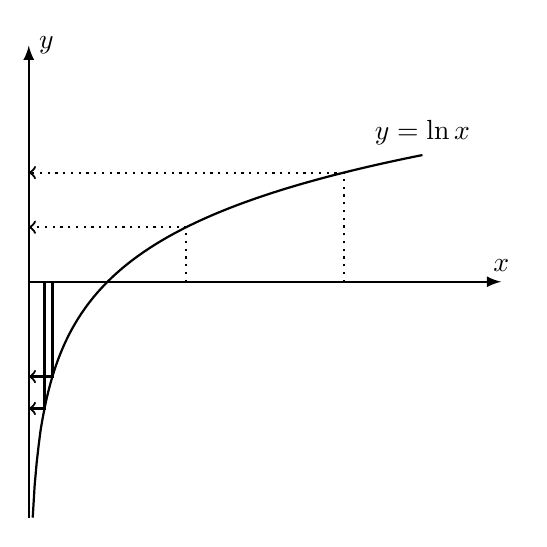
\begin{tikzpicture}[thick]
  \draw[-latex] (0,0) -- (6,0) node[above] {$x$};
  \draw[-latex] (0,-3) -- (0,3) node[right] {$y$};
  \draw[domain=0.05:5, samples=200] plot({\x}, {ln(\x)}) node[above] {$y=\ln x$};
  \draw[->] (0.3,0)--(0.3,-1.204)--(0,-1.204);
  \draw[->] (0.2,0)--(0.2,-1.609)--(0,-1.609);
  \draw[dotted,->] (2,0) -- (2,0.693) -- (0,0.693);
  \draw[dotted,->] (4,0) -- (4,1.386) -- (0,1.386);
\end{tikzpicture}
\end{document}
